%%%%%%%%%%%%%%%%%%%%%%%%%%%%%%%%
\chapter{Sistemas Estocásticos}%
%%%%%%%%%%%%%%%%%%%%%%%%%%%%%%%%

%Motivação do estudo no tema
Existe atualmente uma vasta literatura dedicada ao estudo de sistemas estocásticos, devido à crescente complexidade das aplicações modernas \cite{mixed2010, Djudd12}. O estudo dessa classe de sistemas foi impulsionado em grande parte pelos avanços em telecomunicações e em computação distribuída. Entretanto, os processos estocásticos também estão presentes em diversas áreas da ciência como, por exemplo, economia e biologia \cite{bremaud}.

%Próximas seções
Neste segundo capítulo serão abordados alguns conceitos de sistemas estocásticos, conceitos esses que estão por trás dos modelos apesentados no trabalho. Sendo assim, serão discutidos conceitos relacionados às equações de diferença, matrizes estocásticas e cadeias de Markov \cite{costafragosotodorov,haggs}.

%Portanto, serão apresentadas questões sobre equações de diferença, matrizes estocásticas e cadeias de Markov  serão apresentados afim de proporcionar uma melhor compreensão do trabalho desenvolvido. Ao mesmo tempo é feita uma breve contextualização dos modelos estudados e simulados.


%%%%%%%%%%%%%%%%%%%%%%%%%%%%%%%%%%%
\section{A Equação de Diferença}%
%%%%%%%%%%%%%%%%%%%%%%%%%%%%%%%%%%%

%Modelo do PageRank
A simulação do \textit{PageRank} é dada por uma equação de diferença com vetores e matrizes estocásticas. Cada um dos valores do vetor representa a importância de uma página. A simulação consiste em calcular o próximo vetor de estados, de forma recursiva, até que se atinja um valor estacionário. Assim, o cálculo do \textit{PageRank} é representado pela seguinte equação de diferença de primeira ordem:

\begin{equation} \label{xA}
	x(k+1) = A x(k),\qquad k=0,1,2,\ldots.
\end{equation}


%%%%%%%%%%%%%%%%%%%%%%%%%%%%%%%%%%%%%%%%%%%%%%%%%%%%%%%%%%%%
\section{Definição e Propriedades de Matrizes Estocásticas}%
%%%%%%%%%%%%%%%%%%%%%%%%%%%%%%%%%%%%%%%%%%%%%%%%%%%%%%%%%%%%

Os sistemas estocásticos possuem uma matriz de transição específica, conhecida como matriz estocástica, matriz probabilidade ou ainda matriz de Markov. A matriz estocástica é usada para descrever a transição de uma cadeia de Markov. Cada uma de suas entradas é um número real não negativo representando uma probabilidade de transição. Essas matrizes podem assumir três formatos: o de coluna estocástica, o de linha estocástica e o duplamente estocástica. 

Uma matriz coluna estocástica tem como propriedade ter cada coluna com soma igual a um, matriz A em \eqref{A},

%Trata-se de uma matriz em que todos os elementos são números reais não negativos, cuja soma das linhas e/ou colunas é igual a 1.
%Trata-se de uma matriz $x \in \mathbb{R}^{n \times n}$ em que todos os elementos são números reais não negativos, ou seja, poderia-se ter zeros entre esses elementos, mas não números negativos, $x \geq 0$.

\begin{equation}\label{A}
A = \begin{pmatrix} 
 		\frac{1}{2}	&	\frac{1}{3}	&	0	&	\frac{1}{2}\\
 			0		&	\frac{1}{3}	& 	0	&	\frac{1}{2}\\
 		\frac{1}{2}	&	0			&	1	&	0\\
 			0		&	\frac{1}{3}	&	0	&	0
		\end{pmatrix},
\end{equation}

\noindent e uma matriz linha estocástica tem como propriedade ter cada linha com soma igual a um, matriz B em \eqref{B},

\begin{equation}\label{B}
B = \begin{pmatrix}
 		\frac{1}{2}	&	\frac{1}{2}	&	0			&	0\\
 			0		&	\frac{1}{2}	&	0			&	\frac{1}{2}\\
 			0		&	0			&	1			& 	0\\
 		\frac{1}{4}	&	\frac{1}{4}	&	\frac{1}{4}	&	\frac{1}{4}
		\end{pmatrix}.
\end{equation} 

\noindent Já uma matriz duplamente estocástica tem a propriedade de cada coluna e linha ter soma igual a um, matriz C em \eqref{C},

\begin{equation}\label{C}
C = \begin{pmatrix}
 		 0	&	0			&	0			& 1 \\
 		 0	&	\frac{1}{2}	&	\frac{1}{2}	& 0 \\
 		 0	&	\frac{1}{2}	&	\frac{1}{2}	& 0 \\
 		 1	&	0			&	0			& 0
		\end{pmatrix}.
\end{equation}

\noindent E por fim, o vetor estocástico, ou vetor probabilidade, possui cada um de seus elementos como números reais não negativos e com soma igual a um, vetor v em \eqref{v},

\begin{equation}\label{v}
v = \begin{pmatrix}
	0	\\	\frac{1}{2}	\\	0	\\	\frac{1}{2}
	\end{pmatrix},
\end{equation}

\noindent seguindo o mesmo que para uma matriz de única coluna ou linha.


%%%%%%%%%%%%%%%%%%%%%%%%%%%%%%%%%%%%
%\subsection{Matrizes Não Negativas}%
%%%%%%%%%%%%%%%%%%%%%%%%%%%%%%%%%%%%

%Uma matriz não negativa é primitiva se ela for irredutivel e tiver apenas um autovalor de módulo máximo. Em uma cadeia de Markov, isso corresponde a uma cadeia ser irredutível e aperiódica. E uma matriz $X \in \mathbb{R}^{n \times n}$ é redutível se:

%\begin{itemize}
%\item $n = 1$ e $X = 0$,

%\item ou $n \geq 2$ e existir uma matriz $P \in \mathbb{R}^{n \times n}$ e um $r$ inteiro com $1 \leq r \leq n-1$ tal que:
%
%\begin{equation}
%	P^TXP = \begin{pmatrix}
% 			B & C\\
%			0 & D
%			\end{pmatrix},
%\end{equation}
%
%onde $B \in \mathbb{R}^{r \times r}$, $C \in \mathbb{R}^{r \times (n-r)}$ e $D \in \mathbb{R}^{(n-r) \times (n-r)}$.
%\end{itemize}

%Na seção seguinte são tratadas as questões de cadeias de Markov, e a mudança no modelo do sistema linear, que agora passa a ser um sistema linear com saltos Markovianos.


%%%%%%%%%%%%%%%%%%%%%%%%%%%%
\section{Cadeias de Markov}%
%%%%%%%%%%%%%%%%%%%%%%%%%%%%

%Definição de cadeias de Markov
Os sistemas sujeitos a saltos markovianos pertencem a classe de sistemas estocásticos. Podem se apresentar em tempo contínuo ou discreto. E de forma análoga, podem possuir um espaço de estados contínuos, ou discretos. Neste trabalho, considera-se sistemas lineares cuja transição, ou salto, de uma configuração para outra é representada por uma cadeia de Markov. A cadeia de Markov é um processo estocástico cuja estimação do estado futuro só depende do estado presente. Com isso, dizemos que tal processo de salto não possui memória a respeito de seus estados anteriores.

%O processo estocástico por trás dos sistemas sujeitos a saltos markovianos é a cadeia de Markov, que trata-se de um processo estocástico onde a estimação de um próximo estado só depende do estado presente. Sendo assim, os sistemas sujeitos a saltos markovianos não possuem memória a respeito de seus estados anteriores. 

%Modelo matemático
Assim, considere $\theta = {\theta(k), k = 0,1,...}$ uma cadeia de Markov no espaço de estados discreto $n = {1, 2, … , W}$. Com a seguinte propriedade: 

%\begin{equation}\label{Pij}
%P \bigl( \theta(k+1) = j \mid  \theta(k) = i, \theta(k-1),
%   \ldots, \theta(0)\bigr)
%= P \bigl( \theta(k+1) = j \mid  \theta(k) = i\bigr),
%\end{equation}       

\begin{equation}\label{Pij}
P \bigl( \theta(k+1) = j \mid  \theta(k) = i_k, \theta(k-1) = i_{k-1}, \ldots, \theta(0) = i_0\bigr) =\\
P \bigl( \theta(k+1) = j \mid  \theta(k) = i_k\bigr).
\end{equation}

\noindent denominada propriedade de Markov. Observa-se na propriedade \eqref{Pij}, que no contexto do \textit{PageRank} $i$ trata-se da página onde encontra-se um determinado navegador e $j$ é a página para a qual ele está seguindo. Vale lembrar que o lado direito da igualdade da expressão \eqref{Pij} aparece simplificado pelo fato dos estados anteriores serem irrelevantes para este processo estocástico.   

Uma cadeia de Markov com espaço de estados discreto pode ser interpretada como um grafo. A figura \ref{markovchain} mostra um exemplo desta abordagem. Neste trabalho considera-se que partindo-se de um determinado estado, os estados seguintes a serem alcançados são identicamente prováveis. Portanto, dado que de cada um dos nós $1$,$2$,$3$ e $4$ é possível ir para qualquer outros dois, a probabilidade de ir para cada um dos outros dois seguintes é de $50\%$.

\
\begin{figure}[!htb]
	\centering
	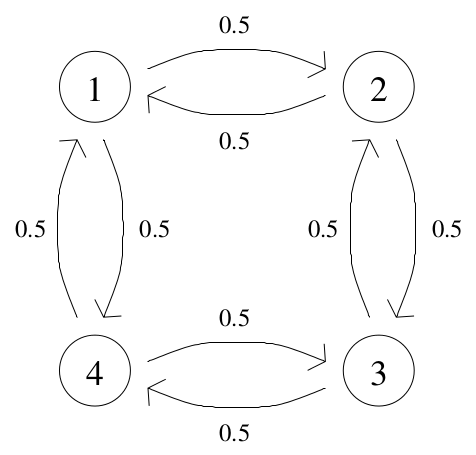
\includegraphics[scale=0.3]{imagens/markovchain}
	\caption{Ilustração de uma simples cadeia de Markov.}
	\label{markovchain}
\end{figure}

\noindent Sendo assim, a matriz estocástica referente ao grafo seria a matriz \eqref{M},

\begin{equation}\label{M}
	D = \begin{pmatrix}
 			0		&	\frac{1}{2}	&	0			&	\frac{1}{2}\\
 		\frac{1}{2}	&	0			&	\frac{1}{2}	&	0\\
 			0		&	\frac{1}{2}	&	0			& 	\frac{1}{2}\\
 		\frac{1}{2}	&	0			&	\frac{1}{2}	&	0
		\end{pmatrix}.
\end{equation} 

\noindent E a simulação em questão seria então dada pela equação \eqref{xBx},

\begin{equation} \label{xBx}
	x(k+1) = D x(k),\qquad k=0,1,2,\ldots.
\end{equation}